\documentclass[a4paper,10pt, twocolumn]{article}
\usepackage[german, english]{babel} % Languages
\usepackage{tikz} % Tikz figures
\usepackage{siunitx} % SI-units package
\usepackage{bm} % Bold mathematics
\usepackage{listings} % Make listings, e.g. for code
\usepackage{enumitem} % Enumerate and itemize commands
\usepackage{multicol} % Make multiple columns for content
\usepackage[left=15mm, right=15mm, bottom=15mm, top=15mm, includeheadfoot]{geometry} % Modify geometry of page format
\usepackage{placeins} % For float barrier command
\usepackage{amsmath} % Math environments
\usepackage{fancyhdr} % Include the fancyhdr package
\usepackage{amsthm} % Theorem environments
\usepackage{siunitx} % Use SI
\usepackage{array} % Use array package for tables
\usepackage{tabularx} % Package to make nice tables
\usepackage{amssymb} % Math symbols
\usepackage{lipsum} % Provide dummy text
\usepackage{abstract} % Abstract package
\usepackage{nicefrac} % Nice fractions in in-line texts
\usepackage[hidelinks]{hyperref} % Make document with hyperlinks
\usepackage{cleveref} % Make references
\usepackage{subcaption} % Make subfigures
\usepackage{graphicx} % Make figures
\usepackage{mhchem} % Chemical notation
\usepackage{mathtools} % Various math tools
\usepackage{framed} % Frame equations
% Figure caption setup
\captionsetup{font=footnotesize,labelfont=bf}

% Python code listings
\definecolor{codegreen}{rgb}{0,0.6,0}
\definecolor{codegray}{rgb}{0.5,0.5,0.5}
\definecolor{codepurple}{rgb}{0.58,0,0.82}
\definecolor{backcolour}{rgb}{0.95,0.95,0.92}

\lstdefinestyle{mystyle}{
	backgroundcolor=\color{backcolour},   
	commentstyle=\color{codegreen},
	keywordstyle=\color{magenta},
	numberstyle=\tiny\color{codegray},
	stringstyle=\color{codepurple},
	basicstyle=\ttfamily\footnotesize,
	breakatwhitespace=false,         
	breaklines=true,                 
	captionpos=b,                    
	keepspaces=true,                 
	numbers=left,                    
	numbersep=5pt,                  
	showspaces=false,                
	showstringspaces=false,
	showtabs=false,                  
	tabsize=2
}

% Enumerate style
\renewcommand{\theenumi}{(\arabic{enumi})}
\renewcommand\labelenumi{\theenumi} % Change enumerate style from 1. to (1) etc.
\renewcommand{\theenumiii}{(\arabic{enumiii})}
\renewcommand\labelenumiii{\theenumiii} % Change enumerate style from 1. to (1) etc.
\setlist{itemsep = 0.2pt}

% Matrix and vector notation
\newcommand\matr[1]{\ensuremath{\boldsymbol{\mathbf{#1}}}}
\newcommand\vect[1]{\ensuremath{\bm{#1}}}
\newcommand\dint{\ensuremath{\int\displaylimits}}

% Units definitions
\DeclareSIUnit \parsec {pc}
\DeclareSIUnit \magnitudes {mag}

% Theorem environment
\newtheorem{tm}{Theorem}
\numberwithin{tm}{subsection}

% New tag form
\newtagform{normalsize}[\normalsize]{\normalsize(}{\normalsize)}

% Configure head- and footlines
\pagestyle{fancy} % Set head- and footlines
\fancyhead[C]{Adult face predicting machine} % Left headline
\fancyhead[L]{\nouppercase{\leftmark}} % Right headline
\fancyhead[R]{D. Zahnd, R. Zahnd}

\author{Daniel Zahnd}
\date{May 14, 2024 - \today}
\title{Benford's law \\ \vspace{0.5cm} \normalsize A heuristic derivation, simulation and explanation of the Newcomb-Benford law}

\begin{document}

%\newgeometry{left=40mm,right=40mm}
\maketitle
%\newpage
%\pagenumbering{roman}
%\tableofcontents
%\FloatBarrier
%\newpage
%\pagenumbering{arabic}
%\setcounter{page}{1}


\begin{abstract}
This paper is concerned with a heuristic derivation of the Benford law from first principles. It is shown in the paper, that the NBL arises from the requirement of scale invariance alone. Scale invariance means, that the mantissa $x$ of a number from a dataset has the same probability $p(x)\,\mathrm{d}x$ of being in the interval $[x, x + \mathrm{d}x]$, as $\lambda x$ has the probability $p(\lambda x)\,\mathrm{d}(\lambda x)$ of being in the interval $[\lambda x, \lambda x + \mathrm{d}(\lambda x)]$ for $\lambda \in \mathbb{R}$. The possible range for $x$ or $\lambda x$ respectively is the interval $[1,10]$.

The derived NBL is applied to a simulated dataset following the the Benford distribution, aswell as to various datasets of different nature.
\end{abstract}

\section{Introduction}
The Benford law was actually discovered by \cite{Newcomb1881}. He observed, that the pages in logarithm books containing tables for logarithms with number one were much dirtier than the pages with logarithms of higher numbers. He proposed that the first digit $1$ is much more likely to occur in a dataset spanning many orders of magnitude than a higher number larger than one. \cite{Benford1938} rediscovered this law later on and formalized it. Only through Theodore Hill however, the Benford law came to be known by a greater mathematical community, because he applied Benford's distribution to solve real world problems.

Nowadays, Benford's law is used to detect frauds in various kinds of datasets. What is important to note here is that the law is only applicable to datasets spanning many orders of magnitude. The reason for this will become more clear with a heuristic derivation given below.


\section{Derivation of the Newcomb-Benford law}
Following \cite{Burgos2021}, Benford's law can be derived from scale invariance. Let $p(x)$ denote the probability density for the mantissa $x$ of some number $z = x\cdot 10^k$ with $k \in \mathbb{Z}$ to be in the interval $[1,10]$. Scale invariance for $p(x)$ then means, that the probability $p(x)\,\mathrm{d}x$ of $x \in [x, \mathrm{d}x]$ is equal to the probability $p(\lambda x)\,\mathrm{d}(\lambda x)$ of $\lambda x \in [\lambda x, \mathrm{d}(\lambda x)]$ for the scaled probability density $p(\lambda x)$. From the normalization condition \begin{align}\begin{aligned}\label{eq:normalizationcondition}
	\int_{1}^{10} p(x)\,\mathrm{d}x =& \int_{1}^{10} p(\lambda x)\,\mathrm{d}(\lambda x) \\ =& \lambda \int_{1}^{10} p(\lambda x)\,\mathrm{d}x \overset{!}{=} 1
	\end{aligned}\end{align}
of probability densities, the relation \begin{equation}
	p(\lambda x) = \lambda^{-1}p(x)
\end{equation} follows. Differentiation \begin{equation}
\frac{\mathrm{d}}{\mathrm{d}\lambda} p(\lambda x) = x\frac{\mathrm{d}p(x)}{\mathrm{d}x}, \qquad \frac{\mathrm{d}}{\mathrm{d}\lambda}[\lambda^{-1}p(x)] = -\frac{1}{\lambda^2}p(x)
\end{equation}
of both sides of \cref{eq:normalizationcondition} leads to the differential equation \begin{equation}
	x\frac{\mathrm{d}p(x)}{\mathrm{d}x} = -\frac{1}{\lambda^2}p(x),
\end{equation} which can be solved by separation of variables. Dividing the differential equation by $x$ and $p(x)$ and furthermore integrating with respect to $x$ leads to \begin{equation}
\int \frac{1}{p(x)}\frac{\mathrm{d}p(x)}{\mathrm{d}x}\,\mathrm{d}x = \int \frac{1}{p(x)}\,\mathrm{d}p(x) =  -\frac{1}{\lambda^2}\int \frac{1}{x}\,\mathrm{d}x.
\end{equation} Performing the indefinite integrals, one obtains \begin{equation}
\ln[p(x)] = -\frac{1}{\lambda^2}\ln(x) + c, \quad c \in \mathbb{R}.
\end{equation} A this stage, one can set $\lambda =1$ and raise both sides of the equation to the power of Euler's number, which yields \begin{equation}
p(x) = \tilde{c}\frac{1}{x},
\end{equation} where $\tilde{c} = e^c$. This constant $\tilde{c}$ is given by the normalization condition $\int_{1}^{10}p(x)\,\mathrm{d}x\overset{!}{=}1$ as \begin{equation}
\tilde{c}\int_{1}^{10}\frac{1}{x}\,\mathrm{d}x = \tilde{c}\ln(10) = 1 \quad \Leftrightarrow \quad \tilde{c} = \frac{1}{\ln(10)},
\end{equation} hence the Benford probability density $p(x)$ is given by \begin{equation}
p(x) = \frac{1}{\ln(10)}x^{-1}.
\end{equation} The probability $P(d)$ that the first digit of a number $z = x\cdot 10^k$ is the integer $d \in \{1,2,\dots,9\}$ is therefore given by \begin{align}\begin{aligned}
P(d) &= \int_{d}^{d+1}p(x)\,\mathrm{d}x = \frac{1}{\ln(10)}\int_{d}^{d+1}\frac{1}{x}\,\mathrm{d}x \\ &= \frac{1}{\ln(10)}[\ln(d+1)-\ln(d)] \\ &= \frac{1}{\ln(10)}\ln\left(1+\frac{1}{d}\right).
\end{aligned}\end{align} Let $a$, $b$ and $c$ be numbers, such that $\log_a(c) = b$ is a well-defined expression. Then, $a^b = c$ holds and hence also $\log_b(a^b) = \log_b(c) = b\log_b(a)$ must hold. From this, the change of basis rule \begin{equation}
\log_a(c) = \frac{\log_b(c)}{\log_b(a)}
\end{equation} follows. Using this rule, one obtains $\ln(10)^{-1} = \log(e)$ and $\ln(1+1/d) = \log(1+1/d)/\log(e)$. Thus, the final expression \begin{equation}
P(d) = \log\left(1 + \frac{1}{d}\right)
\end{equation} for the Newcomb-Benford law is obtained. A dataset $Z \doteq \{z_1,\dots,z_n\}$ consisting of $n \in \mathbb{N}$ numbers is said to follow a Benford distribution, if \begin{equation}
\frac{n_{d}}{n} \approx P(d) = \log\left(1+\frac{1}{d}\right)
\end{equation} for all $d \in \{1,2,\dots,9\}$ holds, where $n_{d}$ is the number of elements in $Z$ with first digit $d \in \{1,2,\dots,9\}$.


\section{Methods}
\subsection{Generated datasets}
This section describes two methods for generating datasets, which should follow a Benford distribution. These methods were implemented and examined as part of this work.

% Briefly explain what this section is about and mention goal

\subsubsection{Method 1: Sampling from uniform distributions}
A method directly derivational on the premiss of scale invariance is based on sampling from uniform distributions of various intervals.
\begin{figure}[h]
	\centering
	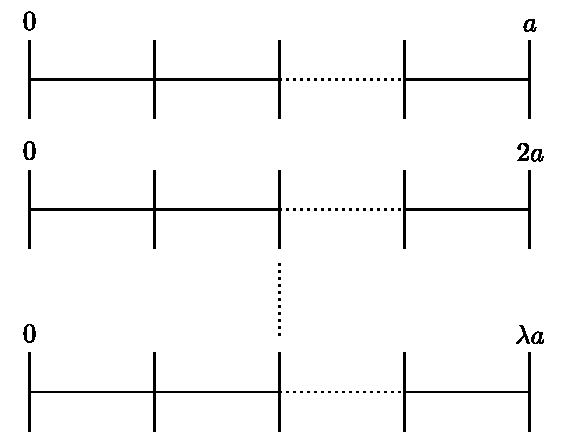
\includegraphics[width=0.3\textwidth]{figures/uniformscale.pdf}
	\caption{Dataset construction by sampling from uniform distributions of intervals $[0,a], [0,2a], \dots, [0,\lambda a]$.}
	\label{fig:uniformscale}
\end{figure}
This method is illustrated with \cref{fig:uniformscale} and is based on drawing samples 
\begin{equation}
	z_{j} \sim U(0,ka), \quad k \in \{1,\dots,\lambda\}
\end{equation}
with $j \in \{1,\dots,n\}$ for $n \in \mathbb{N}$ from uniform distributions $U(0,ka)$. The probability that a sample $z_j$ was drawn from the uniform distribution $U(0,ka)$ is herewith assumed to be \begin{equation}
	P(z_j \sim U[0,ka]) = \frac{1}{k}
\end{equation} to account for the overlap of the various uniform distributions. Given such a construction, one would expect that the resulting dataset should follow a Benford distribution, since it is constructed solely on the assumption of scale invariance.

% Make illustration and explain more into detail

\subsubsection{Method 2: Sampling from a logarithmic uniform distribution}
There is an instructive way to generate a dataset following a Benford distribution. First of all, one has to recall, to which type of data Benford's law applies. Benford's law applies to data spanning many orders of magnitude, since scale invariance was required for the derivation. Data covering many orders of magnitude is typically processed on a logarithmic scale as shown in \cref{fig:logarithmicscale}. Now, an a priori assumption on a dataset spanning many orders of magnitude would be, that it is uniformly distributed over those magnitudes.
\begin{figure}[h]
	\centering
	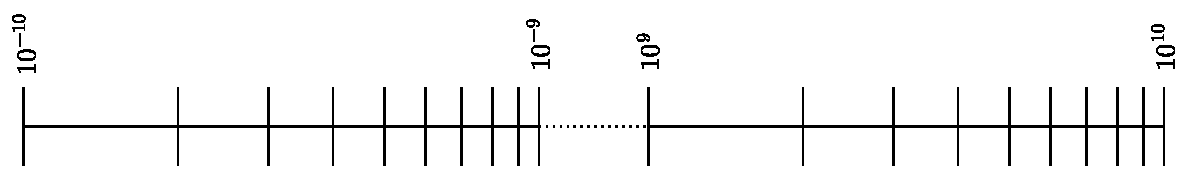
\includegraphics[width=0.4\textwidth]{figures/logarithmicscale.pdf}
	\caption{Logarithmic scale with base 10, ranging from $10^{-10}$ to $10^{10}$.}
	\label{fig:logarithmicscale}
\end{figure}
This is to say, that such a dataset can be generated by sampling data from a range $[10^{r^-}, 10^{r^+}]$ on a logarithmic scale. A sample $z_j$ for $j \in \{1,\dots,n\}$ with $n \in \mathbb{N}$ therefore is obtained as \begin{equation}\label{eq:gensamples}
	z_j = 10^{r_j}, \quad r_j \sim U(r^-,r^+),
\end{equation} where $U(r^-,r^+)$ denotes the uniform distribution between $r
^-$ and $r^+$ for $r^-$, $r^+ \in \mathbb{R}$. For an accordingly generated dataset, $\lim_{n\rightarrow \infty} \frac{n_d}{n} = P(d)$ should hold.

\subsection{World population dataset}
The current section describes the Newcomb-Benford law applied to investigate a real-world dataset, namely a dataset of country populations. The used country population dataset\footnote{Data source: World Bank Open Data, \url{https://data.worldbank.org/indicator/SP.POP.TOTL}, last accessed: June 09, 2024.} features population data for all countries on the world ranging from the period of 1970 to the year 2023. In a first step, only the first digits of country populations of one year (2022) were graphed and compared to the exact Newcomb-Benford law, whereas in a second step all data from 1970 to 2023 was used to compare it against the Benford law.
% Explain data and goal

\subsection{Bible numbers dataset}
This section elucidates the method of the Newcomb-Benford law applied to a dataset of numbers that appear in the Bible. As a basis, the English American Standard Version (ASV) was used. Text files of this translation can be downloaded freely on the internet from various domains. From a text file containing the entire ASV Bible, chapter and verse numbers were removed, as they are not original to the intitial writings, but were added by translators and typewriters at later stages in time. From the resulting text file, all word- and digit-based numbers were extracted into a dataset containing all numbers mentioned in the Bible. Note, that the acquired dataset does not contain numbers used to reference sequential events, such as the word ``fourth'' in the sentence ``...and it was the fourth day...''.


\section{Results}
\subsection{Generated datasets}
This section is concerned with presenting the results obtained for the generated datasets. Some key features and interesting properties are pointed out, which will be discussed in the section below.

\subsubsection{Method 1: Sampling from uniform distributions}
In \cref{fig:gen_method_1}, the results obtained for method 1 of dataset generation are presented, namely those for the sampling from uniform distributions of various intervals. One can see, that for digits $d \in \{1,2,3\}$, the generated dataset seems to have a lower probability of occurrence than the Benford law would predict. However, for digits 4 to 9, the opposite is true; the predicted probabilities as predicted by the NBL are lower in this case than those present in the generated dataset.
\begin{figure}[h]
	\centering
	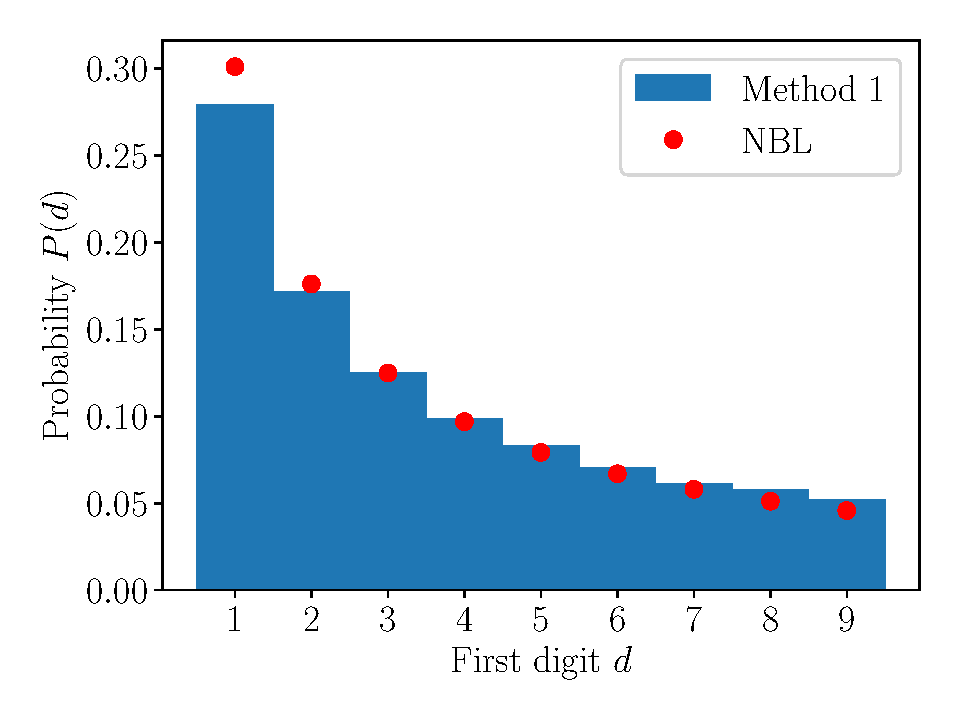
\includegraphics[width=0.4\textwidth]{figures/gen_method_1.pdf}
	\caption{Comparison of the exact Newcomb-Benford law with a generated dataset according to method 1.}
	\label{fig:gen_method_1}
\end{figure}
% Briefly present results and mention most prominent features


\subsubsection{Method 2: Sampling from a logarithmic uniform distribution}
The visualization \cref{fig:gen_method_2} features a histogram showing the distribution of first digits $d$ in the generated dataset according to method 2; namely sampling from a logarithmic uniform distribution. As compared to method 1, this second method provides results even more coherent with the exact Newcomb-Benford law. For all first digits $d \in \{1,\dots,9\}$, the generated dataset seems to follow a Benford distribution very well.

\begin{figure}[h]
	\centering
	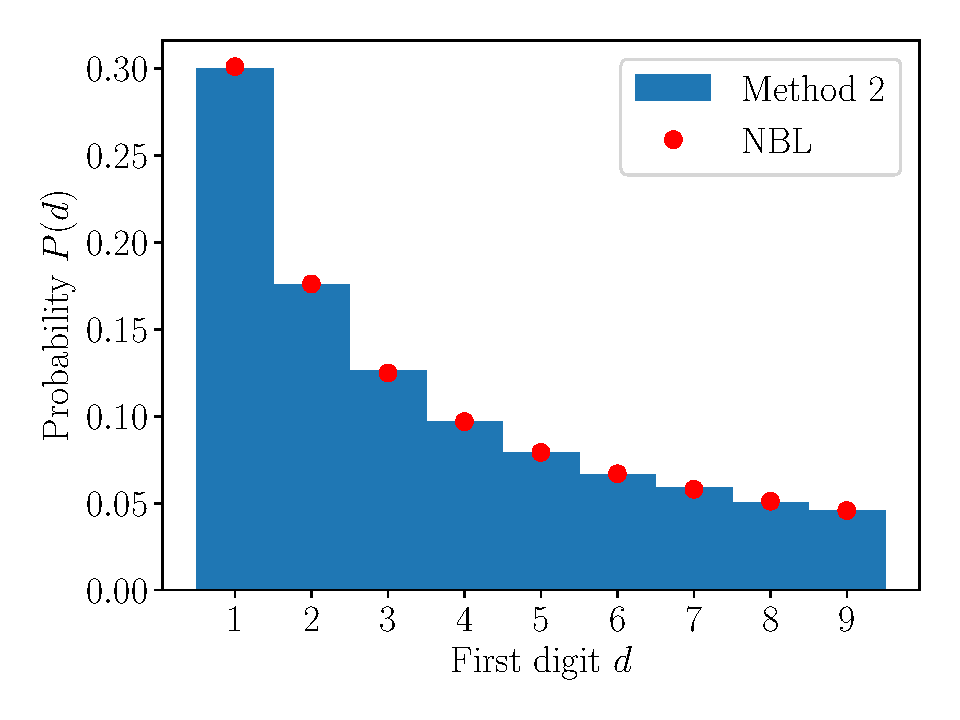
\includegraphics[width=0.4\textwidth]{figures/gen_method_2.pdf}
	\caption{Comparison of the exact Newcomb-Benford law with a generated dataset according to method 2.}
	\label{fig:gen_method_2}
\end{figure}
% Briefly present results and mention most prominent features

\subsection{World population dataset}
The world population data as obtained for only one year seems to only follow a Benford distribution roughly, as \cref{fig:pop_2022} indicates. However, if data of all years present in the used dataset are taken into account, a different picture emerges: The world populations from years 1960 to 2023 seem follow a Benford distribution quite well, as \cref{fig:pop_1960_2023} shows.

The numbers in the world population data for only one year are shown to span a range of 5.8 orders of magnitude, with the highest number being 7950946801 and the lowest 11312. For the dataset containing the populations of all considered years, the numbers span a range of 6.5 orders of magnitude, with highest number 7950946801 and lowest being 2646.
% Briefly present results and mention most prominent features

\begin{figure}[h]
	\centering
	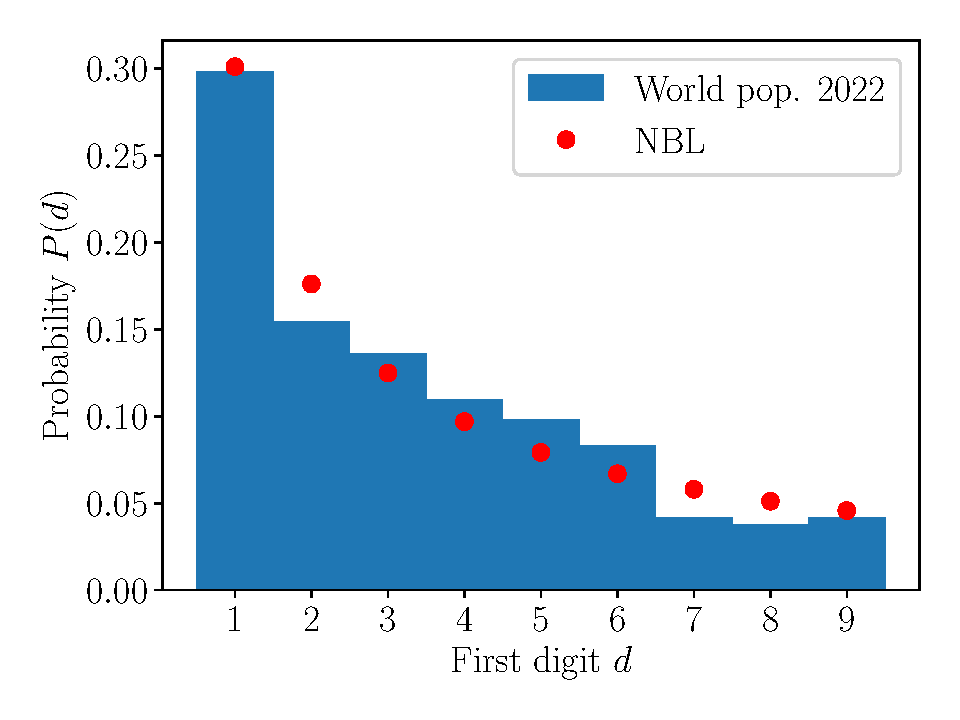
\includegraphics[width=0.4\textwidth]{figures/pop_2022.pdf}
	\caption{Comparison of the exact Newcomb-Benford law with the world population dataset for country populations of the year 2022.}
	\label{fig:pop_2022}
\end{figure}

\begin{figure}[h]
	\centering
	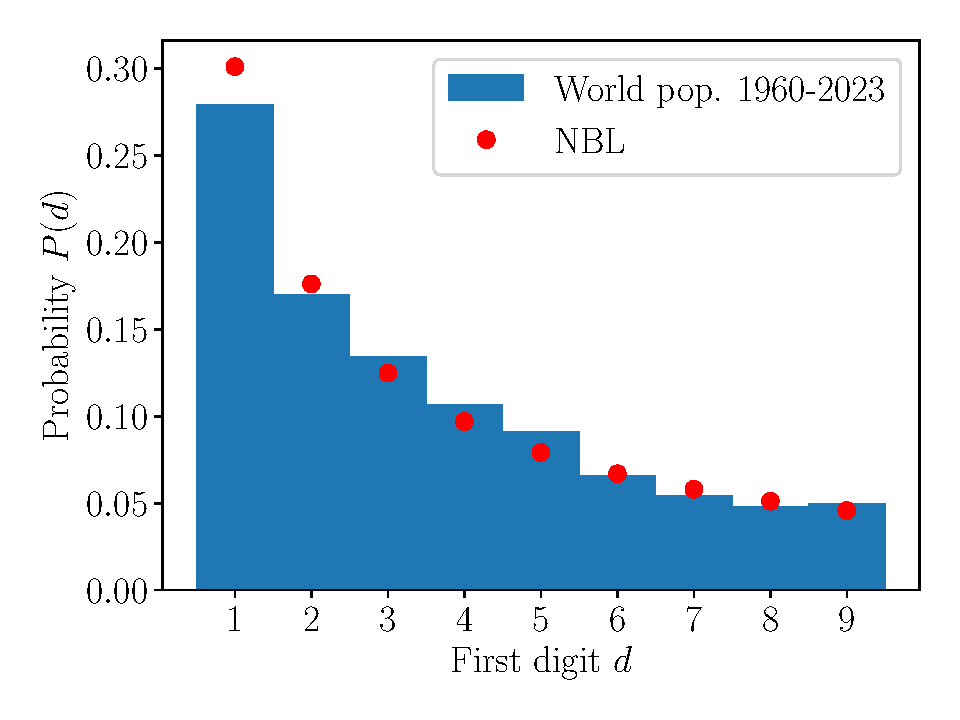
\includegraphics[width=0.4\textwidth]{figures/pop_1960_2023.pdf}
	\caption{Comparison of the exact Newcomb-Benford law with the world population dataset for country populations from 1960 to 2023.}
	\label{fig:pop_1960_2023}
\end{figure}

\subsection{Bible numbers dataset}
The first digits of numbers extracted from the Bible follow a distribution as seen in \cref{fig:bible_numbers}. With respect to the NBL, there is an excess of numbers with first digits 1 and 2, but a shortage of numbers with first digits 3 to 9. The dataset of Bible numbers seems to not match a Benford distribution very well; however, it is observed to follow the general trend predicted by Benford's law, that there should be less numbers with high first digits in a dataset following the Benford distribution. For the first digit 7, there is a spike to be observed in the probability $P(d=7)$ relative to $P(d=6)$ and $P(d=8)$.

The dataset of Bible numbers is shown to feature a range of 5.9 orders of magnitude, with highest number 800000 and lowest number 0.

\begin{figure}[h]
	\centering
	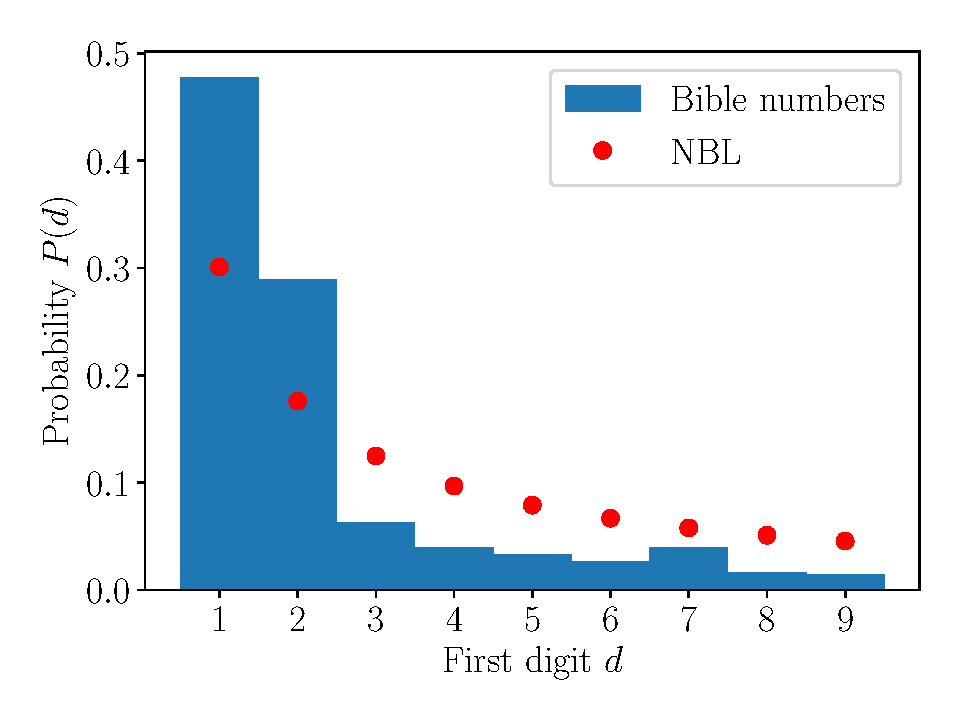
\includegraphics[width=0.4\textwidth]{figures/bible_numbers.pdf}
	\caption{Comparison of the exact Newcomb-Benford law with the dataset containing all numbers from the ASV Bible translation. Note, that numbers refferring to sequential entities such as ``fourth'' in a sentence like ``..it was the fourth...'' are not contained in the dataset.}
	\label{fig:bible_numbers}
\end{figure}

\section{Discussion}
With respect to the two presented methods for generation of Benford distributed datasets one can say, that both methods seem to indeed produce datasets following a Benford distribution. Method 2 hereby provides better agreement with the exact NBL than method 1 does. Likely this could be explained by mathematically showing that the sampling method provides faster convergence to a Benford distributed dataset than method 1. One can propose the conjecture that in the limit $n \rightarrow \infty$ for $n$ the amount of datapoints both methods will lead to exact Benford distribution; this presumption is substantiated by the presented results.

The application of the NBL to real-world data such as the world country populations provides insightful results. It is to be expected from the theory of Benford distributions, that a dataset complying with the requirements of a Benford distribution will approach an exact Benford distribution with increasing size of the dataset. As the world populations dataset matches the Benford distribution requirements, this is indeed what can be seen in the results.

As for the second application of the NBL to real-world data, namely to the Bible numbers, the used dataset proves to not follow a Benford distribution very well. However, the dataset follows the trend as given by the NBL. The observed discrepancies between the probabilities $P(d)$ of first digits $d$ in the Bible numbers dataset and the NBL is likely explained by the presumption, that the dataset does not fulfill the requirements to follow a Benford distribution.

In order for a dataset to follow a Benford distribution, it must contain numbers spanning many orders of magnitude. Over a logarithmic scale of the span of numbers, the numbers in the dataset should furthermore be uniformly distributed. The Bible numbers dataset spans a range of 5.9 orders of magnitude, which is comparable to the dataset of world country populations for one year. However, in the case of the Bible numbers dataset, this span may not be enough. In addition to this, it is not clear if the dataset matches the requirement, that the numbers must be generated by natural processes. Many numbers in the Bible are the product of concious agents such as humans or divine beings. It is hence debatable, if the numbers in the Bible are generated by a purely ``natural'' process.

The peculiar spike for the first digit $d=7$ could be explained by the observation, that the number 7 is special in the Bible: It is the number many theologians believe to be the number of perfection, as God is reported to have instantiated many things that quantify with the number 7.
% Discuss the various features mentioned in the results section


\section{Conclusions}
It was shown in this paper, that there are instructive ways to generate a Benford distributed dataset based only on the assumption of scale invariance. The generated test datasets according to both proposed methods showed a nearly Benford distributed behaviour.

In addition to this, the NBL was successfully applied to a dataset containing world country population numbers. Since this is a dataset spanning many orders of magnitude and because the dataset has natural processes, namely reproduction and migration, at its base, the set is expected to follow a Benford distribution. Indeed, this could be shown in the work at hand.

Furthermore, the NBL was also applied to a somewhat exotic dataset, namely a dataset containing all numbers - except verse and chapter numbers - in the Bible. Since the dataset does not sufficiently fulfill the requirements to a Benford distributed dataset, it does only follow Benford's law to a very coarse approximation. However, the general trend as predicted by the NBL is followed by the dataset, which gives some evidence for the authenticity of the reported numbers in the Bible. That is, if the numbers in the Bible were wholly made up, one would expect to see no correlation between the NBL and te dataset.

In conclusion, Benford's law provides an instructive and most interesting tool to detect, if a dataset spanning many orders of magnitude is of natural origin; that is to say, if natural processes have led to the resulting distribution of first digits in the dataset.
% Draw conclusions from work done

\appendix


%\end{multicols}

\bibliography{references}
\bibliographystyle{apalike}

\end{document}